\section{Continuous Time Stochastic Control}

\subsection{Merton's optimal consumption/investment problem}

Let us now consider the problem of an agent that maximizes consumption utility over his/her lifetime / a fixed horizon. (Brief recap):

Let us consider that his/her wealth $X_t$ evolves according to
\begin{equation*}
    dX_s = \mu(s, X_s, u_s) ds + \sigma(s, X_s, u_s) dW_s
\end{equation*}
with initial condition $X_t = n$. In this formulation:
\begin{itemize}
    \item $u_s = \alpha(s, X_s) \in \mc{U}$ is the control process;
    \item $W_s$ is a \vocab{Brownian Motion} (BM).
\end{itemize}

We assume the SDE has a unique strong solution (i.e., the control $u$ is \vocab{admissible}, denoted by $u \in \mc{U}$).

Let us consider the problem:
\begin{equation*}
    V(t,n) = \sup_{u \in \mc{U}} J_{t,n}(u) = \EE \left[ \int_t^T e^{-\rho(s-t)} f(s, X_s^u, u_s) ds + e^{-\rho(T-t)} g(X_T^u) \right]
\end{equation*}

Then, under some assumptions (regularity, existence of an optimal $u$, ...) the solution to the problem can be found as a solution to the \vocab{HJB Equation}:
\begin{equation}
    \begin{cases}
        \partial_t v(t,n) + \sup_{u \in \mc{U}} \left\{ \tr(\sigma \sigma^T(n,u) D^2 v(t,n)) + \langle \mu(n,u), \nabla v(t,n) \rangle + f(t,n,u) \right\} = \rho v(t,n) \\
        v(T,n) = g(n), \quad n \in \RR^d
    \end{cases}
\end{equation}
where $(t,n) \in [0,T] \times \RR^d$. The HJB equation is a PDE in the unknown function $v(t,n)$.

\subsubsection{Steps to solve the problem:}

\begin{enumerate}
    \item Consider the static optimization problem for arbitrary $(t,n)$ and solve:
    \begin{equation*}
        \sup_{u \in \mc{U}} \left\{ \tr(\sigma \sigma^T(n,u) D^2 v(t,n)) + \langle \mu(n,u), \nabla v(t,n) \rangle + f(t,n,u) \right\}
    \end{equation*}
    treating $t$ and $n$ as fixed parameters and $f, \mu, \sigma \sigma^T, v$ as given functions or parameters.
    
    \item The solution $\hat{u}$ will depend on $t, n$ and $v$:
    \begin{equation*}
        \hat{u} = u(t,n;v)
    \end{equation*}
    
    \item We now need to find $v$. We thus substitute our candidate optimal control $\hat{u}$ into the HJB and solve it.
\end{enumerate}

The $\hat{v}$ we find is the candidate value function and using a verification theorem we can say it is the optimal value function, and $\hat{u} = u(t,n;\hat{v})$ is the optimal control.

\subsection{Market Model with Two Securities}

We consider now a market in which 2 securities are traded:
\begin{itemize}
    \item \vocab{Risk-less} (bank account):
    \begin{equation*}
        dB_t = r B_t dt
    \end{equation*}
    \item \vocab{Risky} (stock):
    \begin{equation*}
        dS_t = \mu S_t dt + \sigma S_t dW_t, \quad S_0 = s
    \end{equation*}
\end{itemize}

The wealth $X_t$ will follow the dynamics:
\begin{equation}
    dX_t = X_t \left[ \pi_t^0 r + \pi_t^1 \mu \right] dt - C_t dt + \pi_t^1 \sigma X_t dW_t \tag{$*$}
\end{equation}
where $(\pi_t^0, \pi_t^1)$ is the \vocab{investment strategy} and $C_t$ is \vocab{consumption}. We require:
\begin{equation*}
    C_t \geq 0; \quad \pi_t^0 + \pi_t^1 = 1 \quad \forall t \geq 0
\end{equation*}

The agent's problem will be:
\begin{equation}
    \max_{\pi^0, \pi^1, C} \EE \left[ \int_0^T e^{-\rho t} f(t, C_t) dt + e^{-\rho T} g(X_T) \right]
\end{equation}
subject to:
\begin{itemize}
    \item Wealth dynamics $(*)$ with $X_0 = n_0$;
    \item $C_t \geq 0$;
    \item $\pi_t^0 + \pi_t^1 = 1 \quad \forall t \geq 0$.
\end{itemize}
Here, $\rho$ is the "subjective" discount factor.

\subsection*{Optimizing Terminal Utility from Wealth}

Let us first consider again the problem of maximizing terminal utility in this context. 

Hence, $C_t = 0 \quad \forall t$, and the performance criterion is $J_{t,n} = \EE \left[ u(X_T^{t,n}) \right]$ for $(t,n) \in [0,T] \times \RR$. 

For simplicity, let us assume no discounting.

First, we have to prove that the value function $v$ is increasing and concave in $n$.

Fix $0 < n \leq y$, and let $\pi_t$ be an admissible control. 
The process $Z_s = X_s^{t,y} - X_s^{t,n}$ satisfies the following SDE:
\begin{equation*}
    dZ_s = Z_s \left[ (\pi_s \mu + (1-\pi_s) r) ds + \pi_s \sigma dW_s \right];
\end{equation*}
Since $Z_t = y - n \geq 0$, it follows that $Z_s \geq 0$ for all $s \geq t$, which implies:
\begin{equation*}
    X_s^{t,y} \geq X_s^{t,n} \quad \forall s \geq t
\end{equation*}

Since the utility function $u$ is increasing, we have $u(X_T^{t,n}) \leq u(X_T^{t,y})$, and consequently:
\begin{equation*}
    \EE \left[ u(X_T^{t,n}) \right] \leq \EE \left[ u(X_T^{t,y}) \right] \leq v(t,y) \quad \forall \pi \in \mc{U}
\end{equation*}
Taking the supremum over $\pi \in \mc{U}$ on the left-hand side shows that $v(t,n) \leq v(t,y)$, so $v$ is increasing in $n$.

Now, consider $n_1, n_2 > 0$, two control processes $\pi^1, \pi^2 \in \mc{U}$, and a constant $\lambda \in [0,1]$.

Consider $n_\lambda = \lambda n_1 + (1-\lambda) n_2$. Let $X^{t,n_i}$ be the wealth process starting from $n_i$ at time $t$ and controlled by $\pi^i$ for $i=1,2$.

Then,
\begin{equation*}
    \pi_s^\lambda = \frac{\lambda X_s^{t,n_1} \pi_s^1 + (1-\lambda) X_s^{t,n_2} \pi_s^2}{\lambda X_s^{t,n_1} + (1-\lambda) X_s^{t,n_2}} \in \mc{U} \text{ by convexity}
\end{equation*}
Consider now $X^\lambda = \lambda X^{t,n_1} + (1-\lambda) X^{t,n_2}$, which evolves according to
\begin{equation*}
    dX_s^\lambda = X_s^\lambda \left[ \pi_s^\lambda \mu + (1-\pi_s^\lambda) r \right] ds + X_s^\lambda \pi_s^\lambda \sigma dW_s
\end{equation*}
\begin{equation*}
    X_t^\lambda = n_\lambda
\end{equation*}
In other words, $X^\lambda$ is a wealth process starting from $n_\lambda$ at $t$ and controlled by $\pi^\lambda$.

Since $u$ is concave:
\begin{equation*}
    u \left( \lambda X_T^{t,n_1} + (1-\lambda) X_T^{t,n_2} \right) \geq \lambda u \left( X_T^{t,n_1} \right) + (1-\lambda) u \left( X_T^{t,n_2} \right)
\end{equation*}
\begin{equation*}
    \Rightarrow J_{t,n_\lambda} \geq \lambda \EE \left[ u \left( X_T^{t,n_1} \right) \right] + (1-\lambda) \EE \left[ u \left( X_T^{t,n_2} \right) \right]
\end{equation*}
$\forall \pi^1, \pi^2 \Rightarrow J_{t,n_\lambda} \geq \lambda J_{t,n_1} + (1-\lambda) J_{t,n_2}$
$\Rightarrow$ the value function is concave in $n$.

\subsection*{Solving the HJB Equation}

We are now ready then to solve the problem. The HJB reads:
\begin{equation*}
    \frac{\partial V}{\partial t} + \sup_{\pi \in \mc{U}} \left[ \mc{L}^\pi V(t,n) \right] = 0, \quad V(T,n) = u(n)
\end{equation*}
where the infinitesimal generator is:
\begin{equation*}
    \mc{L}^\pi V(t,n) = n(\pi \mu + (1-\pi) r) \frac{\partial V}{\partial n} + \frac{1}{2} n^2 \pi^2 \sigma^2 \frac{\partial^2 V}{\partial n^2}
\end{equation*}

Let us consider the \vocab{CRRA utility function} (Constant Relative Risk Aversion: $-n \frac{u''(n)}{u'(n)}$):
\begin{equation*}
    u(n) = \frac{n^\gamma}{\gamma}, \quad n \geq 0, \quad \gamma \neq 0, \gamma < 1
\end{equation*}
Then, it is possible to find an explicit solution to the problem. Let's guess a form for the candidate solution:
\begin{equation*}
    V(t,n) = \phi(t) \cdot u(n)
\end{equation*}
with derivatives:
\begin{align*}
    V_t(t,n) &= \phi'(t) \cdot u(n) \\
    V_n(t,n) &= \phi(t) u_n(n) \\
    V_{nn}(t,n) &= \phi(t) u_{nn}(n)
\end{align*}
where $u_n(n) = n^{\gamma-1}$ and $u_{nn}(n) = (\gamma-1) n^{\gamma-2}$.

Substituting into the HJB we have:
\begin{equation*}
    \phi'(t) \cdot \frac{n^\gamma}{\gamma} + \sup_{\pi \in \mc{U}} \left[ n (\pi \mu + (1-\pi) r) \phi(t) n^{\gamma-1} + \frac{1}{2} n^2 \pi^2 \sigma^2 (\gamma-1) n^{\gamma-2} \phi(t) \right] = 0
\end{equation*}
\begin{equation*}
    \Rightarrow \phi'(t) + \phi(t) \underbrace{\gamma \sup_{\pi \in \mc{U}} \left[ \pi \mu + (1-\pi) r - \frac{1}{2} \pi^2 \sigma^2 (1-\gamma) \right]}_{P} = 0
\end{equation*}
Hence, this is a first order linear ODE, and thus (with boundary condition $\phi(T)=1$):
\begin{equation*}
    \phi(t) = e^{P(T-t)}
\end{equation*}
Thus, the value function is $V(t,n) = e^{P(T-t)} u(n)$.

$V(t,n)$ is strictly increasing and concave in $n$. The term $\pi \mu + (1-\pi) r - \frac{1}{2} \pi^2 \sigma^2 (1-\gamma)$ is strictly concave in $\pi$ and has a maximum at $\hat{\pi}$:
\begin{equation*}
    \text{F.O.C. for } \hat{\pi}: \mu - r - \pi \sigma^2 (1-\gamma) = 0 \Rightarrow \hat{\pi} = \frac{\mu - r}{\sigma^2 (1-\gamma)}
\end{equation*}
and the optimal wealth process evolves as:
\begin{equation*}
    dX_t = X_t (\hat{\pi} \mu + (1-\hat{\pi}) r) dt + \sigma X_t \hat{\pi} dW_t
\end{equation*}

Is the controlled wealth process which admits a unique solution.

\subsection*{\color{red}OPTIMAL CONSUMPTION}

Let's consider the case in which the agent is interested in maximizing his/her (discounted) consumption utility. The objective function is of the form:
\begin{equation*}
    \EE \left[ \int_0^T f(t, c_t) dt \right]
\end{equation*}
with wealth dynamics:
\begin{equation*}
    dX_t = X_t \left[ \pi_t^0 r + \pi_t^1 \mu \right] dt - c_t dt + \pi_t^1 \sigma X_t dW_t
\end{equation*}
subject to:
\begin{equation*}
    \left. \begin{aligned} c_t &\geq 0 \\ \pi_t^0 + \pi_t^1 &= 1 \end{aligned} \right\} \quad \forall t \geq 0. \text{ This defines the set of admissible controls } \mc{U}.
\end{equation*}
We set $\pi_t^1 = \pi_t$ and $\pi_t^0 = 1 - \pi_t$.

\vocab{Problem}: If $f$ is increasing and unbounded, the agent might consume infinitely, causing wealth to become negative, as the current constraints do not prohibit it.

\vocab{Solution}: Consider a fixed domain $D \subseteq [0, T] \times \RR$. If the state process $X$ hits the boundary $\partial D$, the activity is stopped.

Hence, define the stopping time $\tau = \inf \{ t \geq 0 : (t, X_t) \in \partial D \} \wedge T$ and consider the domain:
\begin{equation*}
    D = [0, T] \times \{ n : n > 0 \} \quad \text{\color{red}(we require wealth to be positive, otherwise we stop!)}
\end{equation*}
The performance criterion becomes:
\begin{equation*}
    J_{t,n} = \EE \left[ \int_t^\tau f(s, c_s) ds \right]
\end{equation*}
Rewriting the wealth dynamics $dX_t$:
\begin{align*}
    dX_t &= X_t [(1 - \pi_t) r + \pi_t \mu] dt - c_t dt + \pi_t \sigma X_t dW_t \\
    dX_t &= X_t \pi_t (\mu - r) dt + [X_t r - c_t] dt + \pi_t \sigma X_t dW_t
\end{align*}
The corresponding \vocab{HJB Equation} is:
\begin{equation*}
    \partial_t v(t,n) + \sup_{c, \pi} \left\{ f(t,c) + [\pi n (\mu - r) + nr - c] \partial_n v(t,n) + \frac{1}{2} \sigma^2 \pi^2 n^2 \partial_{nn} v(t,n) \right\} = 0,
\end{equation*}
with boundary conditions:
\begin{align*}
    v(T,n) &= 0 \\
    v(t,0) &= 0
\end{align*}

Let us now consider a \vocab{power utility} function with \vocab{subjective discounting}:
\begin{equation*}
    f(t, c_t) = e^{-\rho t} c^\gamma, \quad \gamma < 1
\end{equation*}
This is a \vocab{CRRA} utility with relative risk aversion:
\begin{equation*}
    R(c) = - \frac{c u''(c)}{u'(c)} = \frac{-c \gamma (\gamma - 1) c^{\gamma-2}}{\gamma c^{\gamma-1}} = 1 - \gamma
\end{equation*}
The static optimization problem inside the HJB is:
\begin{equation*}
    \sup_{\pi, c} \left\{ e^{-\rho t} c^\gamma + [\pi n (\mu - r) + nr - c] \partial_n v(t,n) + \frac{1}{2} \sigma^2 n^2 \pi^2 \partial_{nn} v(t,n) \right\}
\end{equation*}
The \vocab{First Order Conditions (F.O.C.s)} are:
\begin{itemize}
    \item[(a)] For $c$: $e^{-\rho t} \gamma c^{\gamma-1} = \partial_n v(t,n) \implies \gamma c^{\gamma-1} = e^{\rho t} \partial_n v(t,n)$
    \item[(b)] For $\pi$: $n(\mu - r) \partial_n v(t,n) + \pi \sigma^2 n^2 \partial_{nn} v(t,n) = 0 \implies \hat{\pi} = - \frac{\partial_n v(t,n)}{n \partial_{nn} v(t,n)} \cdot \frac{\mu - r}{\sigma^2}$
\end{itemize}

%%%%

We now have to find the function $v$.

We guess it, given the shape of the utility function, as:
\begin{equation*}
    v(t,n) = e^{-\rho t} h(t) n^\gamma
\end{equation*}
Since $v(T,n) = 0$, we have $h(T) = 0$. Here $h'(t)$ is the time-derivative of $h(t)$.
The partial derivatives are:
\begin{align*}
    \partial_t v(t,n) &= e^{-\rho t} h'(t) n^\gamma - \rho e^{-\rho t} h(t) n^\gamma \\
    \partial_n v(t,n) &= \gamma e^{-\rho t} h(t) n^{\gamma-1} \\
    \partial_{nn} v(t,n) &= \gamma(\gamma-1) e^{-\rho t} h(t) n^{\gamma-2}
\end{align*}

The optimal controls become then:
\begin{align*}
    \hat{\pi}(t,n) &= \frac{\mu-r}{\sigma^2} \left( -\frac{\gamma e^{-\rho t} h(t) n^{\gamma-1}}{n \gamma(\gamma-1) e^{-\rho t} h(t) n^{\gamma-2}} \right) = \vocab{$\frac{\mu-r}{\sigma^2(1-\gamma)}$} \quad \text{\color{red}CONSTANT!} \\
    \hat{c}(t,n) &= \left[ \frac{e^{\rho t}}{\gamma} \cdot \gamma e^{-\rho t} h(t) n^{\gamma-1} \right]^{\frac{1}{\gamma-1}} = \vocab{$n h(t)^{\frac{1}{\gamma-1}}$} \quad \text{\color{red}linear in wealth!}
\end{align*}

We now substitute in the HJB and get:
\begin{multline*}
    e^{-\rho t} h'(t) n^\gamma - \rho e^{-\rho t} h(t) n^\gamma + e^{-\rho t} n^\gamma h(t)^{\frac{\gamma}{\gamma-1}} + \\
    + \left[ \frac{\mu-r}{\sigma^2(1-\gamma)} n(\mu-r) + rn - n h(t)^{\frac{1}{\gamma-1}} \right] \gamma e^{-\rho t} h(t) n^{\gamma-1} + \\
    + \frac{1}{2} n^2 \left[ \frac{\mu-r}{\sigma^2(1-\gamma)} \right]^2 \sigma^2 \gamma(\gamma-1) e^{-\rho t} h(t) n^{\gamma-2} = 0
\end{multline*}
Simplifying, we obtain:
\begin{equation*}
    n^\gamma \left\{ h'(t) + h(t) \underbrace{\left[ \frac{\gamma(\mu-r)^2}{\sigma^2(1-\gamma)} + r\gamma - \frac{1}{2} \frac{(\mu-r)^2 \gamma}{\sigma^2(1-\gamma)} - \rho \right]}_{= A} + h(t)^{\frac{\gamma}{\gamma-1}} \underbrace{(1-\gamma)}_{= B} \right\} = 0
\end{equation*}

$\Rightarrow$ This is an ODE which must be solved by $h(t)$:
\begin{equation*}
    h'(t) + A h(t) + B h(t)^{\frac{\gamma}{\gamma-1}} = 0, \quad h(T) = 0
\end{equation*}

This is a \vocab{Bernoulli equation} which can be solved.

\begin{homework*}
    Solve it explicitly. Hint: consider $y(t) = h(t)^{1-\alpha}$ with $\alpha = \frac{\gamma}{\gamma-1}$
    \begin{align*}
        y'(t) &= (1-\alpha) h(t)^{-\alpha} h'(t) \\
        h'(t) &= -A h(t) - B h(t)^\alpha \\
        \Rightarrow y'(t) &= [-A h(t) - B h(t)^\alpha] (1-\alpha) h(t)^{-\alpha} \\
        &= -A (1-\alpha) h(t)^{1-\alpha} - (1-\alpha) B \\
        y'(t) &= -A (1-\alpha) y(t) - (1-\alpha) B \\
        \Rightarrow y'(t) &+ A (1-\alpha) y(t) + (1-\alpha) B = 0
    \end{align*}
    This is \vocab{linear} in $y'$, with $y(T) = 0$.
\end{homework*}

Once solved, it gives an $h(t)$ for which $v$ solves the HJB equation.

\subsection*{\color{red}The case of a random time horizon}

When planning investments, it is reasonable to assume that the agent has an uncertain investment horizon (lifetime). This was originally already present in Merton's 1969 paper.

\begin{equation*}
    V(n) = \sup_{(\pi, c) \in \mc{\Pi} \times \mc{C}} \EE \left[ \int_0^\tau e^{-\rho t} u(c_t X_t^n) dt \right]
\end{equation*}
where $(\pi, c) \in \mc{\Pi} \times \mc{C}$ are \vocab{admissible} controls, with $\mc{C} \subseteq \RR^+$ and the condition $\int_0^\infty |\pi_t|^2 dt + \int_0^\infty c_t dt < \infty$ a.s.

We assume that $\tau$ is a random time independent of the security processes. Its cdf will be:
\begin{equation*}
    F(t) = \PP(\tau \leq t) = \PP(\tau \leq t \mid \mc{F}_\infty)
\end{equation*}
where $\mc{F}_\infty$ is the filtration generated by $W$, the Brownian motion of the stock.

Hence, $V(n)$ can be written as:
\begin{align*}
    V(n) &= \sup_{(\pi, c) \in \mc{\Pi} \times \mc{C}} \EE \left[ \int_0^\infty e^{-\rho t} u(c_t X_t^n) \mathbb{1}_{\{t < \tau\}} dt \right] \\
    &= \sup_{(\pi, c) \in \mc{\Pi} \times \mc{C}} \EE \left[ \int_0^\infty e^{-\rho t} u(c_t X_t^n) (1 - F(t)) dt \right]
\end{align*}

We assume that $\tau$ is \vocab{exponential}:
\begin{equation*}
    1 - F(t) = e^{-\lambda t} \implies V(n) = \sup_{(\pi, c) \in \mc{\Pi} \times \mc{C}} \EE \left[ \int_0^\infty e^{-(\rho + \lambda) t} u(c_t X_t^n) dt \right]
\end{equation*}
Let $\hat{\rho} = \rho + \lambda$. We consider the power utility $u(c) = \frac{c^\gamma}{\gamma}$ with $\gamma \neq 1$ (typically $\gamma < 1, \gamma \neq 0$).

The \vocab{HJB Equation} attached to this problem is:
\begin{equation*}
    \sup_{\pi, c} \left\{ \left[ n((\mu - r)\pi + r - c) \right] \partial_n v + \frac{1}{2} n^2 \pi^2 \sigma^2 \partial_{nn} v + u(cn) \right\} = \hat{\rho} v
\end{equation*}
where $u(cn) = \frac{(cn)^\gamma}{\gamma}$. From the \vocab{First Order Conditions (F.O.C.s)}:
\begin{itemize}
    \item[($\star$)] For $c$: $-\partial_n v + c^{\gamma-1} n^\gamma = 0 \implies \hat{c} = \left( \frac{\partial_n v}{n^\gamma} \right)^{\frac{1}{\gamma-1}}$
    \item[($\star\star$)] For $\pi$: $n(\mu - r) \partial_n v + \pi n^2 \sigma^2 \partial_{nn} v = 0 \implies \hat{\pi} = -\frac{\partial_n v}{n \partial_{nn} v} \cdot \frac{\mu - r}{\sigma^2}$
\end{itemize}

Note that in the HJB above, we can separate the optimizations. The term $\sup_c \{ u(cn) - cn \partial_n v \}$ is the \vocab{Legendre transform} of $u(cn)$.

We look for a solution with the candidate form:
\begin{equation*}
    v(n) = K u(n) = K \frac{n^\gamma}{\gamma} \implies \partial_n v = K n^{\gamma-1}, \quad \partial_{nn} v = K(\gamma - 1) n^{\gamma-2}
\end{equation*}
Substituting into the HJB, and letting $p = \gamma \sup_\pi \left\{ (\mu-r)\pi + r - \frac{1}{2} \pi^2 \sigma^2 (1-\gamma) \right\}$ be the optimized growth rate from the previous section:
\begin{equation*}
    \hat{\rho} K \frac{n^\gamma}{\gamma} = p K \frac{n^\gamma}{\gamma} + \sup_c \left\{ \frac{c^\gamma n^\gamma}{\gamma} - cn K n^{\gamma-1} \right\}
\end{equation*}
The second supremum is attained at $\hat{c} = K^{\frac{1}{\gamma-1}}$, yielding $\frac{1-\gamma}{\gamma} n^\gamma K^{\frac{\gamma}{\gamma-1}}$. Dividing by $\frac{n^\gamma}{\gamma}$:
\begin{equation*}
    \hat{\rho} K = p K + (1-\gamma) K^{\frac{\gamma}{\gamma-1}} \implies \frac{K}{\gamma} (\hat{\rho} - p) - \left[ \frac{K^{\frac{\gamma}{\gamma-1}}}{\gamma} - K^{1 + \frac{1}{\gamma-1}} \right] = 0
\end{equation*}
This simplifies to an equation in the unknown $K$:
\begin{equation*}
    K^{\frac{1}{\gamma-1}} (1-\gamma) = \hat{\rho} - p \implies K = \left( \frac{1-\gamma}{\hat{\rho} - p} \right)^{1-\gamma}
\end{equation*}
where we require $\hat{\rho} - p = \rho + \lambda - p > 0$. We have thus found an explicit solution to the HJB.

\subsubsection*{Remarks:}
\begin{enumerate}
    \item The same problem is faced by a life insurer or a pension fund that invests on behalf of a pensioner who withdraws (consumes) optimally. However, there might be misalignment between the fund manager's and the pensioner's objectives.
    \item The problem can be modified to feature an inflow $a(t)dt$ (from labour income, etc.). Notice that this won't modify the optimal controls' ($\star$ and $\star\star$) general expressions, but obviously modifies the value function $v$.
\end{enumerate}

\subsection*{\color{red}THE CONSUMPTION / INVESTMENT / INSURANCE PROBLEM}

Suppose now that the individual pays an insurance premium to obtain an insured sum $b$ (determined at $t$) which happens as a jump of a Poisson process with intensity $\lambda_t$ upon his/her death. We generalize the above setup in a few directions. While alive, wealth evolves according to:
\begin{equation*}
    dX_t = (r + \pi_t (\mu - r)) X_t dt + \pi_t \sigma X_t dW_t + a_t dt - c_t dt - \lambda_t^* b_t dt
\end{equation*}
In this formulation:
\begin{itemize}
    \item $a_t dt$: \vocab{labour / non-financial income};
    \item $c_t dt$: \vocab{consumption};
    \item $\lambda_t^* b_t dt$: \vocab{insurance premium} (where $\lambda_t^*$ is the mortality rate used to price the contract, which may be different from the actual mortality $\lambda_t$).
\end{itemize}

The objective is to maximize both the utility from consumption and from terminal wealth:
\begin{multline*}
    V(t, X_t) = \sup_{\pi, c, b} \EE \left[ \int_t^T e^{-\int_t^s (\rho + \lambda_u) du} \left[ w_s^\gamma u(c_s) + \lambda_s (w_s^\tau)^\gamma u(X_s + b_s) \right] ds \right. \\
    \left. + e^{-\int_t^T (\rho + \lambda_u) du} \Delta W^\gamma(T) u(X_T) \right]
\end{multline*}
where the term $\lambda_s (w_s^\tau)^\gamma u(X_s + b_s)$ represents the utility \vocab{in case of death}, and the final term represents the \vocab{terminal utility}.

The associated \vocab{HJB Equation} reads:
\begin{multline*}
    \partial_t v(t, n) + \sup_{\pi, c, b} \left\{ \partial_n v(t, n) \left[ r + \pi(\mu - r)n + a_t - c - \lambda_t^* b \right] \right. \\
    \left. + \frac{1}{2} \partial_{nn} v(t, n) \pi^2 \sigma^2 n^2 + w_t^\gamma u(c) + \lambda_t (w_t^\tau)^\gamma u(n + b) \right\} = (\rho + \lambda_t) v(t, n)
\end{multline*}
with boundary condition $v(T, n) = \Delta W^\gamma(T) u(n)$.

Notice that in the supremum, the terms involving $b$ are separated from those with $c$ and $\pi$. Thus, the \vocab{F.O.C.s} for $\pi$ and $c$ are the same as in the case without life insurance (the addition of $a_t$ also does not change these formulas).

The \vocab{F.O.C.} for $c$ is:
\begin{equation*}
    -\partial_n v(t, n) + w_t^\gamma u'(c) = 0 \implies u'(c) = \frac{\partial_n v(t, n)}{w_t^\gamma}
\end{equation*}
This implies that the \vocab{marginal utility of consumption} equals the (rescaled) \vocab{marginal gain of $v$}. The \vocab{F.O.C.} for $b$ is:
\begin{equation*}
    -\partial_n v(t, n) \lambda_t^* + \lambda_t (w_t^\tau)^\gamma u'(n + b) = 0
\end{equation*}

Let us now focus on the \vocab{power utility} case: $u(n) = \frac{n^{1-\gamma}}{1-\gamma}$. We consider the candidate value function (\textit{ansatz}):
\begin{equation*}
    v(t, n) = \frac{1}{1-\gamma} f(t)^\gamma (n + g(t))^{1-\gamma}
\end{equation*}
where $g(t)$ represents the \vocab{human capital} (arising due to the income stream $a_t$).

\subsubsection*{Steps to solve the HJB:}

\begin{enumerate}
    \item \textbf{Evaluate the derivatives of the candidate value function:}
    \begin{align*}
        \partial_t v(t, n) &= \frac{\gamma}{1-\gamma} \left( \frac{n + g(t)}{f(t)} \right)^{1-\gamma} f'(t) + \left( \frac{n + g(t)}{f(t)} \right)^{-\gamma} g'(t) \\
        \partial_n v(t, n) &= \left( \frac{n + g(t)}{f(t)} \right)^{-\gamma} \\
        \partial_{nn} v(t, n) &= -\gamma \left( \frac{n + g(t)}{f(t)} \right)^{-\gamma-1} \frac{1}{f(t)}
    \end{align*}

    \item \textbf{Plug these derivatives into the F.O.C.s:}
    \begin{itemize}
        \item[(a)] \textbf{For $c$:} $-\left( \frac{n + g(t)}{f(t)} \right)^{-\gamma} + w_t^\gamma c^{-\gamma} = 0 \implies \hat{c} = w_t \frac{n + g(t)}{f(t)}$
        \item[(b)] \textbf{For $\pi$:} $\left( \frac{n + g(t)}{f(t)} \right)^{-\gamma} (\mu - r)n - \gamma \left( \frac{n + g(t)}{f(t)} \right)^{-\gamma-1} \frac{1}{f(t)} \pi \sigma^2 n^2 = 0$
        \begin{equation*}
            \implies \hat{\pi} = \frac{1}{\gamma} \frac{\mu - r}{\sigma^2} \frac{n + g(t)}{n}
        \end{equation*}
        \item[(c)] \textbf{For $b$:} $-\left( \frac{n + g(t)}{f(t)} \right)^{-\gamma} \lambda_t^* + \lambda_t (w_t^\tau)^\gamma (n + b)^{-\gamma} = 0$
        \begin{equation*}
            \implies \hat{b} = \left( \frac{n + g(t)}{f(t)} \right) \left( \frac{\lambda_t^*}{\lambda_t} \right)^{-\frac{1}{\gamma}} w_t^\tau - n
        \end{equation*}
    \end{itemize}
\end{enumerate}

\begin{enumerate}
    \item[2.] \textbf{Optimal Investment Strategy ($\hat{\pi}$):}
    \begin{equation*}
        \hat{\pi} = \underbrace{\left( \frac{\mu - r}{\sigma^2 \gamma} \right)}_{\text{Merton's standard}} \cdot \frac{n + g(t)}{n}
    \end{equation*}
    where $g(t)$ is the \vocab{human capital}.

    \item[3.] \textbf{Optimal Insurance Benefit ($\hat{b}$):}
    \begin{equation*}
        \hat{b} = \underbrace{\frac{w_t^\tau}{f(t)}}_{A} \underbrace{\left( \frac{\lambda_t}{\lambda_t^*} \right)^{\frac{1}{\gamma}}}_{B} (n + g(t)) - n
    \end{equation*}
    Notice that $n + \hat{b}$ is the \vocab{total wealth before death} multiplied by two factors.
    
    If $A \times B = 1 \implies \hat{b} = g(t)$, which means the insurance benefit is exactly the \vocab{human capital lost}.
\end{enumerate}

The ratio $\frac{\lambda}{\lambda^*}$ represents the ratio between the objective mortality rate and the pricing insurance rate.
\begin{itemize}
    \item If $\lambda > \lambda^*$, insurance is "cheap" (one should over-insure!).
    \item The higher the ratio $\frac{\lambda}{\lambda^*}$, the higher the optimal benefit $\hat{b}$.
    \item $w_t^\tau$ weights utility at the time of death: $\uparrow w_t^\tau \implies \uparrow \hat{b}$.
    \item $f(t)$ is the preference-adjusted discount factor: $\uparrow f(t) \implies \downarrow \hat{b}$.
\end{itemize}

\subsection*{\color{red}CORPORATE FINANCE MODELS (Morellec, Brumberg \& Rochet, Ch. 1)}

We will study 2 optimal capital structure problems:
\begin{itemize}
    \item optimal debt issuance
    \item optimal dividends
\end{itemize}

Consider a company with the following structure:

\begin{center}
\begin{tabular}{lcl@{\hspace{1.5cm}}lcl}
    \multicolumn{3}{c}{\textbf{Assets}} & \multicolumn{3}{c}{\textbf{Liabilities}} \\
    \text{\scriptsize LIQUID RESERVES} & $\rightarrow$ & $X_t$ & $D_t$ & $\rightarrow$ & \text{\scriptsize DEBT} \\
    \text{\scriptsize MARKET VALUE OF PRODUCTIVE ASSETS} & $\rightarrow$ & $S_t$ & $E_t$ & $\rightarrow$ & \text{\scriptsize EQUITY}
\end{tabular}
\end{center}

We consider $S_t$ to evolve as:
\begin{equation*}
    dS_t = S_t [r dt + \sigma dW_t], \quad S_0 = s
\end{equation*}
with $b$ being the payout rate.

{\color{red}How can we price $D_t$? How can we select optimal how to finance the company?}

Consider $X_t = 0$ and that the firm has a \vocab{nominal debt value} $F$.

\subsection*{\color{red}DEFAULT AT MATURITY (Merton, 1973)}

Then:

\begin{enumerate}
    \item The discounted value of assets is a martingale:
    \begin{equation*}
        \EE \left[ e^{-rT} S_T \right] = S
    \end{equation*}

    \item The value of equity is:
    \begin{equation*}
        E_0 = \EE \left[ e^{-rT} \max(0, S_T - F) \right]
    \end{equation*}
    which corresponds to the \vocab{payoff of a European call option}.

    \begin{center}
    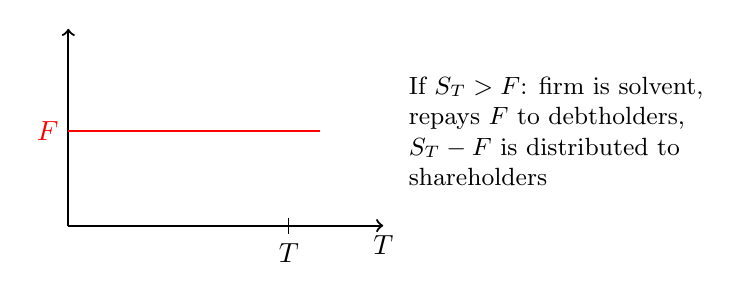
\begin{tikzpicture}[scale=1.0]
        % Axes
        \draw[->, thick] (0,0) -- (4,0) node[below] {$T$};
        \draw[->, thick] (0,0) -- (0,2.5);
        
        % Horizontal line at F
        \draw[red, thick] (0,1.2) -- (3.2,1.2);
        \node[left, red] at (0,1.2) {$F$};
        
        % T tick
        \draw (2.8, 0.1) -- (2.8, -0.1) node[below] {$T$};

        % Text next to diagram
        \node[anchor=west, align=left, font=\small] at (4.2, 1.2) {
            If $S_T > F$: firm is solvent, \\
            repays $F$ to debtholders, \\
            $S_T - F$ is distributed to \\
            shareholders
        };
    \end{tikzpicture}
    \end{center}

    \item The value of debt is:
    \begin{align*}
        D_0 &= \EE \left[ e^{-rT} \min(F, S_T) \right] \\
        &= \EE \left[ e^{-rT} (S_T - \max(0, S_T - F)) \right]
    \end{align*}
    and $E_0 + D_0 = \EE \left[ e^{-rT} S_T \right] = S$.
\end{enumerate}

Given an assumption ($S$ is \vocab{GBM}), $E_0$ and $D_0$ can be found using the Black-Scholes option pricing formula.

\subsection*{\color{red}DEFAULT BEFORE DEBT MATURITY (Black and Cox, 1976)}

Suppose now that shareholders can decide to stop paying debt coupons (and determine default) prior to maturity.

$\rightarrow$ we specify an exogenous \vocab{default BOUNDARY} (at no cost) $\{B_t, t \in [0, T]\}$ and \vocab{LIQUIDATION} is triggered whenever $S_t \leq B_t$.

\subsection*{\color{red}Price of a bond with finite maturity}

How do we price a bond described above?

\begin{equation*}
    \text{Define } \eta = \min \{\tau, T\}, \quad \tau := \inf \{t \geq 0 : S_t = B_t\}
\end{equation*}
\begin{equation*}
    \text{and } \quad p(\eta) = \begin{cases} B_\eta & \text{if } \eta < T \\ F(S_\tau) & \text{if } \eta = T \end{cases}
\end{equation*}

\begin{equation*}
    \text{Then } \quad P(t, S) = \EE \left[ \int_t^\eta e^{-r(l-t)} \underbrace{C(l, S_l)}_{\text{coupon}} dl + e^{-r(\eta-t)} p(\eta) \;\middle|\; S_t = S \right]
\end{equation*}

Given an assumption ($S$ is \vocab{GBM}), $E_0$ and $D_0$ can be found using the Black-Scholes option pricing formula.

\subsection*{\color{red}DEFAULT BEFORE DEBT MATURITY (Black and Cox, 1976)}

Suppose now that shareholders can decide to stop paying debt coupons (and determine default) prior to maturity.

$\rightarrow$ we specify an exogenous \vocab{default BOUNDARY} (at no cost) $\{B_t, t \in [0, T]\}$ and \vocab{LIQUIDATION} is triggered whenever $S_t \leq B_t$.

\subsection*{\color{red}Price of a bond with finite maturity}

How do we price a bond described above?

Define $\eta = \min \{\tau, T\}$, $\tau := \inf \{t \geq 0 : S_t = B_t\}$ and
\begin{equation*}
    p(\eta) = \begin{cases} B_\eta & \text{if } \eta < T \\ F(S_\tau) & \text{if } \eta = T \end{cases}
\end{equation*}

Then
\begin{equation*}
    P(t, S) = \EE \left[ \int_t^\eta e^{-r(l-t)} \underbrace{C(l, S_l)}_{\text{coupon}} dl + e^{-r(\eta-t)} p(\eta) \;\middle|\; S_t = S \right]
\end{equation*}

%%%
which, using the \vocab{Feynman-Kac formula}*, can be associated to the following free-boundary problem:
\begin{equation} \tag{$*$}
\begin{cases}
    \underbrace{rP(t,S)}_{\text{\color{blue}L.H.S. of $(*)$}} = \underbrace{\overbrace{\partial_t P(t,S) + rS\partial_S P(t,S) + \frac{\sigma^2 S^2}{2} \partial_{SS} P(t,S)}^{\text{\color{red}EXPECTED CAPITAL GAINS}} + \underbrace{C(t,S)}_{\text{\color{red}COUPON}}}_{\text{\color{red}FLOW OF EXPECTED GAINS OF HOLDING DEBT}}, & 0 \leq t \leq T; \ S \geq B_t; \\
    P(t, B_t) = B_t; \quad P(T, S) = F(S)
\end{cases}
\end{equation}

By \vocab{no arbitrage}, the R.H.S. of $(*)$ must equal the flow of income obtained by investing $P(t,S)$ at the riskless rate (the L.H.S. of $(*)$).

\begin{center}
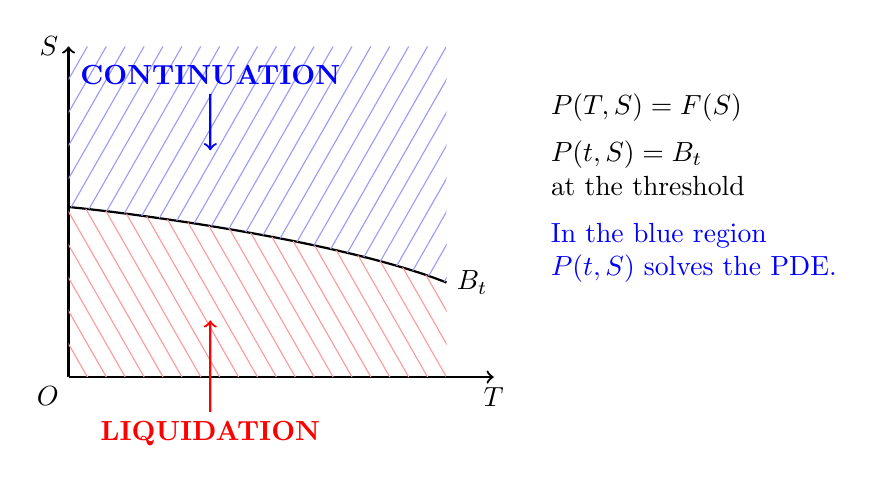
\begin{tikzpicture}[scale=1.2]
    % Axes
    \draw[->, thick] (0,0) -- (4.5,0) node[below] {$T$};
    \draw[->, thick] (0,0) -- (0,3.5) node[left] {$S$};
    \node[below left] at (0,0) {$O$};

    % Boundary curve B_t
    \draw[thick] (0,1.8) .. controls (1,1.7) and (3,1.4) .. (4,1) node[right] {$B_t$};

    % Shaded regions with hatching
    \begin{scope}
        \clip (0,1.8) .. controls (1,1.7) and (3,1.4) .. (4,1) -- (4,3.5) -- (0,3.5) -- cycle;
        \foreach \i in {-2,-1.8,...,6}
            \draw[blue!40, thin] (\i,0) -- (\i+2,3.5);
    \end{scope}

    \begin{scope}
        \clip (0,1.8) .. controls (1,1.7) and (3,1.4) .. (4,1) -- (4,0) -- (0,0) -- cycle;
        \foreach \i in {-2,-1.8,...,6}
            \draw[red!40, thin] (\i,3.5) -- (\i+2,0);
    \end{scope}

    % Labels and arrows
    \node[blue, font=\bfseries] (cont) at (1.5, 3.2) {CONTINUATION};
    \draw[blue, ->, thick] (cont) -- (1.5, 2.4);
    
    \node[red, font=\bfseries] (liq) at (1.5, -0.6) {LIQUIDATION};
    \draw[red, ->, thick] (liq) -- (1.5, 0.6);

    % Text next to diagram
    \node[anchor=west, align=left] at (5, 2) {
        $P(T,S) = F(S)$ \\[0.5em]
        $P(t,S) = B_t$ \\ at the threshold \\[0.5em]
        {\color{blue}In the blue region} \\ {\color{blue}$P(t,S)$ solves the PDE.}
    };
\end{tikzpicture}
\end{center}

\subsection*{\color{red}* FEYNMAN-KAC FORMULA (see Øksendal, or Shreve, for instance)}

\begin{itemize}
    \item It establishes a link between \vocab{stochastic processes} and \vocab{PDEs}.
\end{itemize}

In particular, for boundary value problems, the function
\begin{equation*}
    h(n) = \EE^n \left[ \int_0^{\tau_D} e^{-\int_0^t q(X_s) ds} g(X_t) dt + e^{-\int_0^{\tau_D} q(X_s) ds} \phi(X_{\tau_D}) \right]
\end{equation*}
solves
\begin{equation*}
    \begin{cases}
        \mc{L}h(n) - q(n)h(n) = -g(n) & \text{on } D \\
        \lim_{n \to y} h(n) = \phi(y) & y \in \partial D
    \end{cases}
\end{equation*}
where $\phi$ is bounded and $g$ satisfies $\EE^n \left[ \int_0^{\tau_D} |g(X_s)| ds \right] < \infty$.

%% Page 42

\subsection*{\color{red}Price of a consol bond ($T = +\infty$)}

Consider $C(t, S) = C$, $T = +\infty \rightarrow$ \vocab{CONSOL BOND}, and $B_t = S_B > 0$. Its price $D(S)$ is given by the system:
\begin{equation*}
    \begin{cases}
        rD(S) = rS\partial_S D(S) + \frac{\sigma^2}{2} S^2 \partial_{SS} D(S) + C \\
        D(S_B) = S_B
    \end{cases}
\end{equation*}

{\color{red}This is an ODE (the problem is stationary)} and thus the price can be found by solving it. The associated homogeneous differential equation has the general solution:
\begin{equation*}
    f(S) = K_1 S^{\gamma_1} + K_2 S^{\gamma_2}
\end{equation*}
where $\gamma_1, \gamma_2$ solve the characteristic equation:
\begin{equation*}
    r = r\gamma + \frac{\sigma^2}{2} \gamma(\gamma - 1), \quad \text{with } \gamma_1 < 0 < \gamma_2.
\end{equation*}
Since $\frac{C}{r}$ is a particular solution of the ODE, the general solution is:
\begin{equation*}
    D(S) = K_1 S^{\gamma_1} + K_2 S^{\gamma_2} + \frac{C}{r}
\end{equation*}

$K_1$ and $K_2$ can be found by observing that, when $S \to \infty$, the bond must approach its nominal value:
\begin{equation*}
    \int_0^\infty C e^{-rt} dt = \frac{C}{r} \implies D(\infty) \to \frac{C}{r}.
\end{equation*}
Since $\gamma_1 < 0 < \gamma_2$, this implies that $K_2 = 0$. $K_1$ is then determined by the boundary condition $D(S_B) = S_B$:
\begin{equation*}
    K_1 S_B^{\gamma_1} + \frac{C}{r} = S_B \implies K_1 = S_B^{1-\gamma_1} - \frac{C}{r} S_B^{-\gamma_1}
\end{equation*}
Substituting back, we obtain:
\begin{align*}
    D(S) &= \left[ S_B^{1-\gamma_1} - \frac{C}{r} S_B^{-\gamma_1} \right] \cdot S^{\gamma_1} + \frac{C}{r} \\
    &= \left( \frac{S}{S_B} \right)^{\gamma_1} \left[ S_B - \frac{C}{r} \right] + \frac{C}{r}.
\end{align*}

\begin{homework*}
    \begin{enumerate}
        \item Similarly, price the equity.
        \item How should equityholders choose $S_B$ optimally?
    \end{enumerate}
\end{homework*}

\subsection*{\color{red}DYNAMIC TRADE-OFF THEORY (How to choose $F$? or $C$? or $S_B$?)}
\textit{(Leland, 1994)}

Why do firms issue debt? Trade-off theory says it is because the interests are \vocab{TAX DEDUCTIBLE}.

Suppose the firm's debt is a consol bond with coupon $C$. Shareholders choose the default threshold $S_B$:
\begin{equation*}
    \tau := \inf \{t > 0 : S_t \leq S_B\}
\end{equation*}

The firm pays taxes $\theta \in [0,1]$ on the operating income $\beta S_t$ (where $\beta$ is the payout rate), net of coupon payments:
\begin{equation*}
    T = \theta [\beta S_t - C] \implies (1-\theta)(\beta S_t - C) \text{ is the flow to shareholders.}
\end{equation*}

At date $\tau$, the firm is liquidated and debtholders get $(1-\alpha) S_B$, where $\alpha \in [0,1]$ represents \vocab{DEFAULT COSTS}. The asset value evolves as:
\begin{equation*}
    \frac{dS_t}{S_t} = \mu dt + \sigma dW_t, \quad \mu := r - \beta
\end{equation*}

Then:
\begin{equation*}
    D(S) = \EE \left[ \int_0^\tau e^{-rt} C dt + e^{-r\tau} (1-\alpha) S_B \;\middle|\; S_0 = S \right]
\end{equation*}
$D$ satisfies the free-boundary problem we characterized above:
\begin{equation*}
    \begin{cases}
        rD(S) = \mu S D'(S) + \frac{\sigma^2}{2} S^2 D''(S) + C, & S > S_B \\
        D(S_B) = (1-\alpha) S_B, \quad D(S) \to \frac{C}{r} \text{ as } S \to +\infty
    \end{cases}
\end{equation*}

The value of equity is:
\begin{equation*}
    E(S) = \EE \left[ (1-\theta) \int_0^\tau e^{-rt} (\beta S_t - C) dt \;\middle|\; S_0 = S \right]
\end{equation*}
which gives the following problem:
\begin{equation*}
    \begin{cases}
        rE(S) = \mu S E'(S) + \frac{\sigma^2}{2} S^2 E''(S) + (1-\theta)(\beta S - C), & S > S_B \\
        E(S_B) = 0, \quad E(S) \sim (1-\theta)\left(S - \frac{C}{r}\right) \text{ as } S \to +\infty
    \end{cases}
\end{equation*}

\begin{homework*}
    Solve these problems explicitly. In particular, show that:
    \begin{equation*}
        D(S) = \frac{C}{r} - \left[ \frac{C}{r} - (1-\alpha) S_B \right] \left( \frac{S}{S_B} \right)^{\gamma_1}
    \end{equation*}
\end{homework*}

\begin{equation*}
    E(S) = (1-\theta) \left[ S - \frac{C}{r} + \underbrace{\left( \frac{C}{r} - S_B \right) \left( \frac{S}{S_B} \right)^{\gamma_1}}_{\text{\vocab{LIMITED-LIABILITY OPTION}}} \right]
\end{equation*}

{\color{red}We now consider that $C, S_B$ are chosen optimally:}

\begin{enumerate}
    \item The firm chooses $C$
    \item Debt is issued (at price $D_0$)
    \item Shareholders set $S_B$ (maximizing shareholder value!)
\end{enumerate}
They do not commit ex-ante: they select it ex-post to maximize their value (and creditors anticipate it).

$S_B$ is chosen to maximize $E(S)$ (or, equivalently, the value of the LL option):
\begin{equation*}
    \max_{S_B} \left[ \frac{C}{r} - S_B \right] \cdot S_B^{-\gamma_1}
\end{equation*}
This defines a link between $C$ and $S_B$!
\begin{equation*}
    \rightarrow -\gamma_1 \frac{C}{r} S_B^{-\gamma_1-1} + S_B^{-\gamma_1}(1-\gamma_1) = 0 \implies S_B = \frac{\gamma_1}{\gamma_1-1} \frac{C}{r} < \frac{C}{r}
\end{equation*}
Hence, this is what creditors expect!

\begin{enumerate}
    \item[2)] $D_0$ can be found using debt's valuation formula:
    \begin{equation*}
        D_0 = \frac{C}{r} - \left[ \frac{C}{r} - (1-\alpha) S_B \right] \left( \frac{S}{S_B} \right)^{\gamma_1}
    \end{equation*}
    \item[3)] Suppose that the total investment needed at time 0 to start the firm is $I$.
\end{enumerate}

Then, shareholder's value at $t=0$, i.e., the difference between equity value and the amount that shareholders have invested in the firm is:
\begin{align*}
    SV_0 &= E_0 - (I - D_0) \quad \text{\color{red}(if $I=0$, this is $D_0 + E_0$!)} \\
    &= (1-\theta) \left[ S - \frac{C}{r} + \left( \frac{C}{r} - S_B \right) \left( \frac{S}{S_B} \right)^{\gamma_1} \right] - I + \frac{C}{r} - \left[ \frac{C}{r} - (1-\alpha) S_B \right] \left( \frac{S}{S_B} \right)^{\gamma_1} \\
    &= \underbrace{(1-\theta)S - I}_{\text{NPV of earnings after-tax}} + \underbrace{\theta \frac{C}{r} \left[ 1 - \left( \frac{S}{S_B} \right)^{\gamma_1} \right]}_{\text{expected tax rebate}} - \underbrace{(\alpha - \theta) S_B \left( \frac{S}{S_B} \right)^{\gamma_1}}_{\text{expected net liq costs}}
\end{align*}

$SV_0$ must be maximized given the optimal choice of $S_B$, $S_B^*$, i.e., with $S_B = S_B^* = \frac{\gamma_1}{\gamma_1-1} \frac{C}{r}$.

Indeed,
\begin{equation*}
    SV_0(S_B^*) = (1-\theta)S - I + \frac{\gamma_1-1}{\gamma_1} S_B^* \left[ \theta + \frac{\theta - \alpha \gamma_1}{\gamma_1-1} \left( \frac{S}{S_B^*} \right)^{\gamma_1} \right]
\end{equation*}

Shareholder value is maximized with
\begin{equation*}
    SV_0'(S_B^*) = 0 \rightarrow \frac{\gamma_1-1}{\gamma_1} \theta + \frac{\theta - \alpha \gamma_1}{\gamma_1-1} S^{\gamma_1} (1-\gamma_1) (S_B^*)^{-\gamma_1} = 0
\end{equation*}
\begin{equation*}
    (S_B^*)^{-\gamma_1} = \frac{1-\gamma_1}{\gamma_1} \theta \cdot \frac{1}{1-\gamma_1} S^{-\gamma_1} \frac{\gamma_1-1}{\theta - \alpha \gamma_1}
\end{equation*}
\begin{equation*}
    S_B^* = S \left[ \frac{\theta}{\gamma_1} \frac{\gamma_1-1}{\theta - \alpha \gamma_1} \right]^{-\frac{1}{\gamma_1}}
\end{equation*}

\subsection*{\color{red}OPTIMAL DIVIDENDS (Jeanblanc \& Shiryaev 1995)}

Consider $X$ to be the liquid \vocab{reserves} $X = (X_t)_{t \geq 0}$ of a company with no investment. Reserves are not remunerated and there is no debt.
\begin{equation*}
    dX_t = \underbrace{\mu dt + \sigma dW_t}_{\substack{\text{CUMULATIVE} \\ \text{NET EARNINGS}}} - dz_t, \quad X_0 = n \geq 0, \quad \mu, \sigma > 0
\end{equation*}
where $W_t$ is a standard Wiener process. The term $\mu dt + \sigma dW_t$ is an \vocab{ABM} (Arithmetic BM).
The process $z_t$ is a non-decreasing, adapted \vocab{DIVIDEND PAYMENT STRATEGY}.
We have $dX_t = dz_t = 0$ when $t \geq \tau$, where $\tau$ is the time of \vocab{bankruptcy}.

The company (managers) maximize shareholder's value and are risk-neutral (alternatively, they could maximize utility from dividends):
\begin{equation*}
    V(n) = \sup_z \EE_n \left[ \int_0^\infty e^{-\rho t} dz_t \right]
\end{equation*}
Note that:
\begin{equation*}
    \int_0^\infty e^{-\rho t} dz_t = z_0 + \int_{(0, \infty)} e^{-\rho t} dz_t
\end{equation*}

The objective is to find the supremum over all admissible dividend processes $z = (z_t)_{t \geq 0}$.

\begin{remark}
    We consider $Z$ such that $dZ_t = u(X_t) dt, Z_0 = z_0(n)$.
    
    Suppose $u$ and $z_0$ are measurable functions such that $0 \leq u(n) \leq K < \infty$ (this is the \vocab{bounded case}) and $0 \leq z_0(n) \leq n$. The dynamics of the process $X_t$ are given by:
    \[ dX_t = (\mu - u(X_t)) dt + \sigma dW_t, \]
    which has a unique strong solution. 
    
    Also, we consider $\tau$ as the \vocab{bankruptcy time}, i.e.,
    \[ \tau = \inf \{t : X_t = 0\}, \quad \text{s.t. } X_t = 0 \ \forall t \geq \tau. \]
    
    Let us assume $z_0 = 0$. Then the value function is defined as:
    \[ V(n) = \sup_{0 \leq u(n) \leq K} \EE_n \int_0^\tau e^{-\rho t} u(X_t) dt. \]
    
    As usual, we want to find $\tilde{V}(n)$ using \vocab{Bellman's equation} (and then verify that it is optimal). We thus look for an admissible $u$ that solves:
    \[ \sup_{0 \leq u \leq K} \left[ \mc{L}_u \tilde{V}(n) + u \right] = \rho \tilde{V}(n) \]
    where the generator is $\mc{L}_u \tilde{V}(n) = (\mu - u) \partial_n \tilde{V} + \frac{1}{2} \sigma^2 \partial_{nn} \tilde{V}$. This leads to:
    \[ \mu \partial_n \tilde{V} + \frac{1}{2} \sigma^2 \partial_{nn} \tilde{V} - \rho \tilde{V} + \sup_{0 \leq u \leq K} \left[ u(1 - \partial_n \tilde{V}) \right] = 0. \]
    
    Hence, given $\tilde{V}$, the optimal control $\tilde{u}(n)$ is given by:
    \[ \tilde{u}(n) = \begin{cases} K & \text{if } 1 - \partial_n \tilde{V} \geq 0 \\ 0 & \text{if } 1 - \partial_n \tilde{V} < 0 \end{cases} \]
    
    For $n$ such that $\tilde{u}(n) = 0$, it must hold:
    \[ \mu \partial_n \tilde{V}(n) + \frac{1}{2} \sigma^2 \partial_{nn} \tilde{V}(n) - \rho \tilde{V}(n) = 0, \]
    while if $\tilde{u}(n) = K$ we have:
    \[ \mu \partial_n \tilde{V}(n) + \frac{1}{2} \sigma^2 \partial_{nn} \tilde{V}(n) - \rho \tilde{V}(n) + K(1 - \partial_n \tilde{V}(n)) = 0. \]
    
    Intuitively, given the structure of $\tilde{u}$, there exists a threshold $\tilde{n}$ such that for $n \geq \tilde{n}$ dividends are paid out at maximal possible speed, and $u(n) = 0$ for $n < \tilde{n}$. 
    
    Hence, the solution features a \vocab{free boundary} $\tilde{n}$ such that:
    \begin{align*}
        \mu \partial_n \tilde{V}(n) + \frac{\sigma^2}{2} \partial_{nn} \tilde{V}(n) - \rho \tilde{V}(n) &= 0 \quad \text{if } n < \tilde{n} \tag{*} \\
        (\mu - K) \partial_n \tilde{V}(n) + \frac{\sigma^2}{2} \partial_{nn} \tilde{V}(n) - \rho \tilde{V}(n) + K &= 0 \quad \text{if } n \geq \tilde{n} \tag{**}
    \end{align*}
\end{remark}

Hence, given $\tilde{V}$,

\begin{remark}
    The optimal control $\tilde{u}(n)$ is given by:
    \[ \tilde{u}(n) = \begin{cases} K & \text{if } 1 - \partial_n \tilde{V} \geq 0 \\ 0 & \text{if } 1 - \partial_n \tilde{V} < 0 \end{cases} \]
    For $n$ s.t. $\tilde{u}(n) = 0$, it must hold:
    \[ \mu \partial_n \tilde{V}(n) + \frac{1}{2} \sigma^2 \partial_{nn} \tilde{V}(n) - \rho \tilde{V}(n) = 0, \]
    while if $\tilde{u}(n) = K$ we have
    \[ \mu \partial_n \tilde{V}(n) + \frac{1}{2} \sigma^2 \partial_{nn} \tilde{V}(n) - \rho \tilde{V}(n) + K \left( 1 - \partial_n \tilde{V}(n) \right) = 0. \]
    Intuitively, given the structure of $\tilde{u}$, there exists a $\tilde{n}$ s.t. for $n \geq \tilde{n}$ dividends are paid out at maximal possible speed, and s.t. $u(n) = 0$ for $n < \tilde{n}$.
    
    Hence, the solution features a \vocab{free boundary} $\tilde{n}$ s.t.
    \begin{align*}
        \mu \partial_n \tilde{V}(n) + \frac{\sigma^2}{2} \partial_{nn} \tilde{V}(n) - \rho \tilde{V}(n) &= 0 \quad \text{if } n < \tilde{n} \tag{*} \\
        (\mu - K) \partial_n \tilde{V}(n) + \frac{\sigma^2}{2} \partial_{nn} \tilde{V}(n) - \rho \tilde{V}(n) + K &= 0 \quad \text{if } n \geq \tilde{n} \tag{**}
    \end{align*}
\end{remark}

\begin{remark}
    For (**), we have
    \[ V''(n) + \frac{\mu - \kappa}{\frac{\sigma^2}{2}} V'(n) - \frac{p}{\frac{\sigma^2}{2}} V(n) + \frac{K}{\frac{\sigma^2}{2}} = 0 \]
    which is a $2^{\text{nd}}$ order ODE. Its general solution is
    \[ V(n) = C_1 e^{\lambda_1 n} + C_2 e^{\lambda_2 n} + \frac{K}{p} \]
    with $\lambda_1, \lambda_2$ solving
    \[ \lambda^2 + \frac{\mu - \kappa}{\frac{\sigma^2}{2}} \lambda - \frac{p}{\frac{\sigma^2}{2}} = 0 \]
    \[ \implies \lambda_{1,2} = \frac{\frac{\kappa - \mu}{\frac{\sigma^2}{2}} \pm \sqrt{\left(\frac{\mu - \kappa}{\frac{\sigma^2}{2}}\right)^2 + 4 \frac{p}{\frac{\sigma^2}{2}}}}{2} \]
    Notice that $\lambda_1 > 0, \lambda_2 < 0$ and hence since $\tilde{V}(n) \leq \frac{K}{p}$ because $u(n) \leq K$, $C_1 = 0$!
\end{remark}

%%%%
\begin{remark}
    $\implies V(n) = \frac{K}{p} + C_2 e^{\lambda_2 n}$,
    
    and $C_2 \leq 0$ because $V(n)$ non-decreasing:
    \[ \frac{K}{p} + \lambda_2 C_2 e^{\lambda_2 n} \geq 0 \]
    \[ \implies \lambda_2, C_2 \leq 0 \text{ both!} \]
    
    Instead, when $n < \check{n}$, the function satisfies
    \[ (*) \to \frac{1}{2} \sigma^2 \partial_{nn} \tilde{V}(n) + \mu \partial_n \tilde{V}(n) - p \tilde{V}(n) = 0 \]
    Hence, it is of the form
    \[ V(n) = A_1 e^{r_1 n} + A_2 e^{r_2 n} \]
    with $r_1, r_2$ solving
    \[ r^2 + \frac{\mu}{\frac{\sigma^2}{2}} r - \frac{p}{\frac{\sigma^2}{2}} = 0, \quad D = \Delta \]
    \[ r_{1,2} = \frac{-\frac{\mu}{\frac{\sigma^2}{2}} \pm \sqrt{\left(\frac{\mu}{\frac{\sigma^2}{2}}\right)^2 + \frac{p}{\frac{\sigma^2}{2}}}}{2} \]
\end{remark}

